\chapter{Background}

% SIDDATA (mit Educational Resources dabei, muss kein sub-chapter sein)
% Conceptual Spaces (What is this?)
% Required techniques and algorithms

\section{Replication and Software Quality}

Having established the goals of replicating an algorithm for a new domain, let us look at how such a replication should be performed and how software quality can be measured.

\subsection{Replication and Reproducibility}
\label{sec:howtoreplicate}

\todoparagraph{this field of work seems constrained to a small community, without any alternative implementations or substantial improvements from outside of it.}

The workflow of data science generally follows the same pattern: A paper states there is some problem \textit{X}, claims that their algorithm \textit{Y} may be good at problem \textit{X}, creates datasets \textit{Z} for \textit{X}, and then tests the code on these datasets. This test generally compares \textit{X} to alternative approaches from the literature and explores if any regularities in the algorithm \textit{Y} can be found. This may yield future research opportunities, showing what other domains the algorithm may work for as well.

Replication fills this role by applying an existing algorithm to another domain. Results for this are important, as it helps to see first if the claimed results are valid, and if they work on datasets that are not artificial and specifically created for the sole purpose of testing the algorithm. Furthermore, the details of experiments in publsihed work are often opaque and omit important information to reproduce the algorithm. These issues are mitigated trough repetition: The robustness of the algorithm to changes in parameters or dataset is investigated. If changes in either of these have a major impact on the results, there is reason to doubt generalization of the algorithm, showing that it may not be good to solve problem \textit{X} after all.

It is absolutely crucial in science to ensure that all claims that are made are reproducible and testable, ensuring ease of replication. Reproducibility is the pinnacle of \textit{Open Science}.\footnote{There is no single definition of open science, however reproducibility appears in most tries, such as \eg \url{https://www.talyarkoni.org/blog/2019/07/13/i-hate-open-science/}, accessed at \date{2022}{03}{25}} And \q{Open Science is just science done right}.\footnote{Quote from John Tennant, see \eg \url{https://soundcloud.com/tidningen-curie/jon-tennant-open-science-is-just-science-done-right}, accessed at \date{2022}{03}{25}} Reproducibility refers to the Ability to reproduce - computationally or experimentally - the methods used to produce a given result, by virtue of being accessible and understandable. Being a hot topic in psychology since the reproducibility crisis,\footnote{Baker M: 1,500 scientists lift the lid on reproducibility. Nature. 2016; 533(7604): 452-4. \url{https://www.nature.com/articles/533452a}} the topic is just es relevant in computer science research.\footnote{Mesirov JP: Computer science. Accessible reproducible research. Science. 2010; 327(5964): 415-6. \url{https://www.ncbi.nlm.nih.gov/pmc/articles/PMC3878063/}} In that realm, Reproducibility may be seen as sub-goal of (the more fundamental) Sustainability, as \eg by \textcite{Molder2021a}, who claim that \q{reproducibility alone is not enough to sustain the hours of work that scientists invest in crafting data analyses}.

To ensure that the analysis performed in this thesis is sustainable and adheres to best scientific and software quality standards, let us look at at ways to formally define such.

\subsection{Software Quality}
\label{sec:reproducibility}

The International Organization for Standardization (ISO) provides an official international standard for the evaluation of software quality as \textbf{ISO/IEC 25010:2011} \cite{2013ISOI}. The full title of the norm is \textit{ISO/IEC 25010:2011 Systems and software engineering - Systems and software Quality Requirements and Evaluation (SQuaRE)}. It has the objective to ensure the quality of software by providing objective and clearly defined standards for definitions of success regarding of software products. It classifies software quality in eight characteristics, which each consists of several sub-characteristics. The main characteristics are \textit{Functional Suitability, Performance Efficiency, Compatibility, Usability, Reliability, Security, Maintainability} and \textit{Portability}. Not all of these are relevant to projects like this, such as \textit{Security}, which mostly measures the ability to track actions and identity of users. 

What is needed here are those goals relevant for sustainable data analysis. In this realm, the stated metrics align much with the hierarchy of aspects to consider for sustainable data analysis as published by \textcite{Molder2021a}, which is is reprinted as \autoref{fig:snakemake_aspect_hierachy}.

\begin{figure}[H]
	\centering
	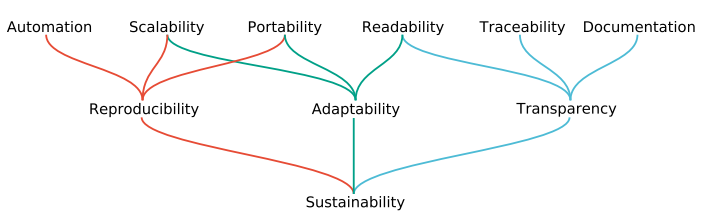
\includegraphics[width=0.7\textwidth]{graphics/stolenfigures/snakemake_aspect_hierachy.png}
	\slcaption{
		Hierarchy of aspects to consider for sustainable data analysis. Reproduced from {\cite[Fig.1]{Molder2021a}} (Creative Commons Attribution License) \label{fig:snakemake_aspect_hierachy}
	}
\end{figure}

Some important aspects to conduct proper computer science and data analysis that allows for \textbf{Sustainability} - allowing the analysis to be of lasting impact - thus include \cite{Molder2021a, 2013ISOI}:

\begin{description}
    \item[Functional Suitability] which means complete, correct and appropriate functionality.
	\item[Reproducibility] \ie allowing validation and regeneration of results on the original or even new data. This understandable and well documented code (also \textit{Changeability and Stability})
	\item[Maintainability and Adaptability] the ability to modify the analysis to answer extended or slightly different research questions by allowing modifications.
	\item[Transparency] \ie the ability for others to understand it well enough to judge if it's technically as well as methodologically valid - also ensuring Understandability, Appropriateness and Accessibility, Analyzability and Testability.
	\item[Scalability] \ie enabling the scalable execution of the algorithm and each involved step, including deployment on complex compute clusters, grids or clouds. This includes Performance Efficiency and efficient Resource Utilization.
	\item[Modularity] \ie changes in one component have a minimal impact on others allowing for easy exchange and extension.
\end{description}


% \begin{description}
%     \item[Functional Suitability], assessing the existance of a set of functions that satisfy the stated needs. It includes \textit{Functional Completeness, Functional Appropriateness (Suitability)} \textit{and Functional Correctness (Accuracy)}
%     \item[Performance Efficiency], assessing the relationship between the performance and the amount of resources used, specifially \textit{Time behaviour, Resource Utilization} and \textit{Capacity}
%     \item[Compatibility], consisting of \textit{Co-Existence and Interoperability}
%     \item[Usability], assessing the effort needed for use, measured by \textit{Appropriateness Recognizability (Understandability), Learnability, Operability, User Error Protection, Accessibility} and \textit{Interface Aesthetics (Attractiveness)}
%     \item[Reliability], assessing the capacity of software to maintain its level of performance, comprising \textit{Maturity, Fault tolerance, Recoverability} and \textit{Availability}
%     \item[Security], among others allowing to track actions and identity: \textit{confidentiality, integrity, non-repudiation, accountability} and authenticity
%     \item[Maintainability], assessing the effort needed to make modifications, which includes \textit{Analyzability, Testability, Modularity} (meaning changes in one component have a minimal impact on others), \textit{reusability} and \textit{modifiability (Changeability+Stability)}
%     \item[Portability], measruing the ability to be transferred to other environments: \textit{Adaptability, Installability} and \textit{Replaceability}
% \end{description}

% Some important aspects to conduct proper (computer) science and data analysis that allows for \textbf{Sustainability} (such that the analysis is of lasting impact), may thus be \cite{Molder2021}:
% \begin{description}
% 	\item[Reproducibility] \ie allowing validation and regeneration of results on the original or even new data. Requiring understandable and well documented code.
% 	\item[Adaptability] \ie the ability to modify the analysis to answer extended or slightly different research questions.
% 	\item[Transparency] \ie the ability for others to understand it well enough to judge if it's technically as well as methodologically valid.
% 	\item[Scalability] \ie enabling the scalable execution of the algorithm and each involved step, including deployment on complex compute clusters, grids or clouds. 
% \end{description}

% Principles of open science are very important to me, so I want to ensure that the claims I am making in this thesis are backed by code that is scalable, reproducible, modular, easily-understood, easily set up and run, well documented, ... . To support this, I will as often as necessary refer to the actual code in this thesis, to allow to understand and reproduce the claims and results, and also highly encourage to critically read everything here and check the respective code (...and let me know if you spot any errors! Just open a Github Issue!)



\section{SIDDATA and Educational Resources}
\label{sec:siddata}

\todoparagraph{Educational resources has no definition, aber siddata ist ein beispiel projekt was darum revolviert}

"Frage war ja, Lässt sich der Algo auf die Domäne von Ed.Res. beziehen, und dafür muss ich sie erklären"

\todoparagraph{auf die kategorien in} \ref{tab:siddata_metadata} hinaus: in principle könnnen educaitonal resources können auch transkribierte videos sein, PDFs als vorlesungsmaterial, ganze paper oder bücher, oder multimedia-data such as in a mooc). \todoparagraph{Hier ider in dataset-section}


% \includeMD{pandoc_generated_latex/2_0_siddata}

To get a better understanding of the domain, this section elaborates on the specific use case of recommendation of education resources that shall be handled, and introduces the SIDDATA project and platform under which this thesis was developed.\footnote{As \textsc{Siddata} signifies both the project and the developed digital assistant, the all-upper 'SIDDATA' henceforth refers to the project, while the specific developed software will be denoted 'Siddata' or 'DSA'.}

This thesis was started while working at the SIDDATA project, with the idea to add a recommender to the platform that can generate course recommendations with the user \textit{in the loop}. SIDDATA is a joint interdisciplinary project for \q{\emph{Individualization of Studies through Digital, Data-Driven Assistants}}\footnote{\url{https://www.siddata.de/en/}} of the universities Osnabrück, Bremen and Leibniz Universität Hannover, funded by the German \emph{Federal Ministry of Education and Research}.\footnote{BMBF. Funding number: 16DHB2124} 

The project adresses the same problem as stated in the Introduction (\ref{sec:many_resources}), namely that e-learning and the amount of avilable resources increase, making the choice of right resources an increasingly relevant problem for the learning success of students. Its deliverable is a flexible data-driven \gls{dsa}, that supports students in higher education in their invidual learning and achievement of personal study goals by giving hints, reminders and recommendation for their individual study paths \cite{Schurz2021}, helping students in setting and achiving individual and self-regulated personal educational goals. This is in line with the increasing importance of skills such as self-organized knowledge acquisition and self-regulatory competencies due increasing importance of individualization in educational paths of the globalized learning environment \cite{Ehlers2019,Schurz2021}.

For that, the collaborative project combines heterogenous data and information in a digital study assistant. Data is collected from multiple sources, such as the \gls{lms}, offers and resources of other universities and institutions, and data collected from its users. To allow for this heterogeniety and also future extensions, for example new data sources  such as \glspl{mooc} through several apis APIs, different front-ends, or different recommendation methods, the system relies on a highly modular and extensible architecture. The Frontend is realized as plugin for the  the university's \gls{lms} Stud.IP \cite{stockmann2005}. This not only allows for easy user access, but also to get data about courses from the LMS using cronjobs. The Frontend is connected over a RESTful API to the Backend, which is written in Python on basis of the Web Framework \textit{Django} and relies on a relational \textit{PostgreSQL} database to store information.

The Backend consists of seperate encapsulated recommender modules in a loosely coupled architecture and a common ontology, allowing to easily add new subsystems. The modules generate recommendations towards personal educational goals on basis of the collected data, which are displayed to the user in the Frontend. What comprises a recommender is grouped from a user perspective, such that each each recommender focuses on a topic. The currently implemented recommenders include for example one to find peers with similar interests, get information about scientific careers, personality-based learning behaviour- and study tips, or information regarding local and remote courses and \glspl{oer}. Another module recommends courses using a combination of rule-based and modern \gls{ml} techniques that relate natural language queries with the courses known to the system (picked up in \autoref{sec:sidbert}) \cite{Schurz2021}.

The system is currently in its third prototype, and preliminary evaluation has shown that modules that provide personal recommendation are most well received \cite{Schurz2021}. This and the ease of use to add new recommenders indicate a high likelyhood of success for adding a new module that recommends courses in the way as described above.

The dataset used here was collected through the Siddata platform as well, which collected courses and events from the three universities currently connected to it, as well as other sources for \glspl{mooc} and other \glspl{oer} through respective APIs. More details in \autoref{sec:dataset_siddata}. It should be noted that the dataset is not artificially generated (unlike \mainalgos) but collected from current courses and their descriptions - making an algorithm for this domain incorporated as recommender to the platform a contribution with practical application.



\section{Conceptual Spaces}
\label{sec:cs}

This section will introduce conceptual spaces as tool of choice as well as how to generate them and how reasoning on them works, as well as some other related work to what's done in this thesis.

\subsection*{Theory of Conceptual Spaces}

The theory of Conceptual Spaces was first introduced by Peter Gärdenfors in his 2000 book \citetitle{Gardenfors2000a} \cite{Gardenfors2000a} both as a theoretical model of human concept formation, but also as format for knowledge representation in artificial systems \cite{Gardenfors2004}. 

On the one hand, \glspl{cs} should serve as bridge between symbolistic and connectionistic approaches to knowledge representation. By having CS as layer of reasoning and representation in between both, classical symbols would be grounded in noisy high-dimensional data, allowing for high-level syllogistic reasoning from real-world data. 

If a computer has a knowledge base that says $\exists x.Red(x) \& Apple(x)$, does it know what "red" and "apple" mean? We need to ground symbols, to express meaning!

According to Gärdenfors, concept-representation in humans is represented by three levels of accounting for observations: The symbolic level, the conceptual level and the subconceptual level \cite[204]{Gardenfors2000a}:
\begin{description}
    \item[Subconceptual] Observations are the firing of the neurons of our sensory receptors, without any conceptualization.  (connectionism, \glspl{ann})
    \item[Conceptual] Observations are defined not as token of a symbol, but as vector in a conceptual space of some quality  (prototype theory, linear algebra)
    \item[Symbolic] represents observations by describing them in some specified language (formal logic, syllogisms, symbolism, classical AI, logical positivism)
\end{description}

These levels are not in conflict, but different models of the same phenonemon, each covering distinct important aspects and each allowing a set of algorithms. The process of inducing a general rule from few samples for example is represented as pattern-matching on the firing patterns in the subconceptual level, which translates to the conceptual level as geometric reasoning through regions and direction. As another example, semantic relations such as hyponyms from the symbolic level are modelled as geometric sub-regions on the conceptual level. So on the one hand, automatically generated conceptual spaces could allow for high-level syllogistic reasoning on real-world data without the need to manually add countless facts. However it also provides a new way to model reasoning and inference for both other levels through geometric relations, providing explanations for the noisy subconceptual level and computationally less complex algorithms for the symbolic level. The validity of the statement \textit{a robin is a bird} is given because robins are gemmetrically a subregion of the region of birds.

Summarized, rregardless of the theory's aspiration to accurately model human conceptualization and reasoning, it provides a useful knowledge representation method and tool that allows to model kinds of human reasoning with novel algorithms that cannot be done with both other well-researched methods \cite[Sec.~6.7]{Gardenfors2000a}. Furthermore it can serve as representational format to express semantic relations for the semantic web \cite{Gardenfors2004} with a richer structure than classical ontologies (\eg RDS, OWL or WordNet) and thus allowing more than deductive reasoning and based on strict is-a relationships and explicit, unambiguous, universal truths.

\subsection*{Definition}

In conceptual spaces, concepts are represented as convex regions in domain-specific, human-interpretable spaces. \autoref{fig:apple_cs} represents a sample space for the concept of \textit{apple}, such that every instance of an apple is thus a vector that lies inside the region of the concept. This allows for high-level reasoning: The question \textit{\q{Will an apple fit into my bag?}} can be answered by checking if the \textit{size} dimension of the region is smaller than the dimension of the bag.

\begin{figure}[H]
	\centering
	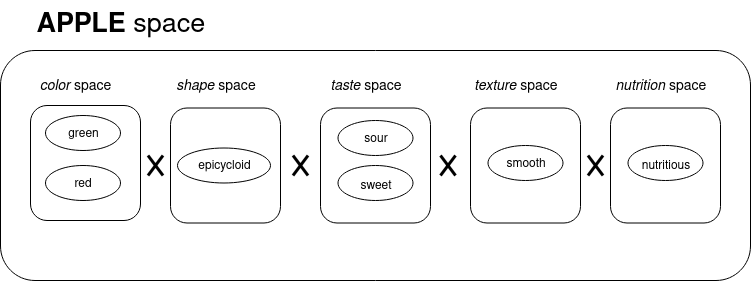
\includegraphics[width=\textwidth]{graphics/stolenfigures/apple_space.png}
	\caption[Inner form of a Conceptual Space for an apple]{
		Inner form of a Conceptual Space for an apple, displayed as product of different properties, which are convex regions in different quality domain spaces. Adapted from \cite{Fiorini2013}.
	}
    \label{fig:apple_cs}
\end{figure}



\fbox{\begin{minipage}{40em}
    \newtheorem*{theorem*}{Conceptual Space}
    \begin{theorem*}
        A conceptual space is a geometric structure used to encode the meaning of natural language terms, properties and concepts. The metric space is spanned by \emph{quality dimensions} denoting basic domain-specific properties based on perception or sub-symbolic processing. Natural language categories (\emph{concepts}) correspond to convex regions, whereas points denote individual objects (instances/\emph{entities}, allowing for geometric solutions to commonsense reasoning tasks such as \emph{betweeness} or \emph{induction}.
        % \cite{Derrac2015}: "Conceptual spaces \cite{Gardenfors2000a} are metric spaces which are used to encode the meaning of natural language concepts and properties."
    \end{theorem*}
\end{minipage}}
\label{sec:csdefinition}


Formally defined, a conceputal spaces needs the following definitions:
\begin{description}
    \item[Quality Dimensions] are atomic units of perception. Some of these are necessarily linked (such as hue and saturation), making them \textit{integral}, whereas others (\eg. temperature and weight) are \textit{seperable}. Typically each dimension corresponds to a primitive cognitive feature.
    \item[Domain] A set of integral dimensions that are seperable from others, like the \textit{color} domain made up from hue, saturation and value. Conceptual spaces are grouped into several low-dimensional subspaces according to these domains.
    \item[Similarity] is defined as inverse distance, which requries a metric. A distinction can be made for the aggregation of integral and separable dimensions. 
    \item[Betweenness] An object Y is between two other objects X and Z iff d(x,y) + d(y,z) = d(x,z).
    \item[Natural Properties (\textit{criterion P} \cite{Gardenfors2000a})] are defined as convex regions of a domain in a conceptual space. A convex region has the property that an interpolation between any two points in this region is necessarily also in this region. 
    \item[Concepts (\textit{criterion C} \cite{Gardenfors2000a})] are combinations of (potentially correlated) properties. \q{A concept is represented as a set of convex regions in a number of
    domains together with a prominence assignment to the domains and information about how the regions in different domains are correlated} \cite[8]{Gardenfors2004}
    \item[Entities] are specific instances (tokens) of a concept, encoded as points. 
    \item[Context] can be modelled in a CS by weighting certain dimensions higher than others, influencing distance and how concepts are fromed from properties.
\end{description}

Some corollaries: 

\begin{itemize}
    \item Each conceptual space contains only items for which the space's dimensions make sense, so you wouldn't find kings in a conceptual space of cabbages.
    \item Concepts roughly correspond to (non-proper) nouns, adjectives to properties and proper nouns (the name of a particular person, place, organization, or thing to points.)
    \item From the criterion of convexity for natural properties and the definition of betweenness, it follows that if an object Y is between X and Z, and both X and Z have a property, Y must also have this property.
    \item Relative properties can be defined as regions on a relative scale - the property "\textit{tall}" acccordingly can be defined to be true iff the entity is in the top 33\% \wrt the size-property of all relevant objects.
\end{itemize}

% \includeMD{pandoc_generated_latex/2_2_conceptualspaces}
\todoparagraph{look if I want to take a paragraph from 22conceptualspacesMD}

\subsection{Data-Driven Generation of Conceptual Spaces}
\label{sec:generate_cs}

So far, the area of application for Conceptual Spaces has been small. Most of the current works that rely on conceptual spaces create custom \textit{phenonemal} spaces for semantic domains, where quality dimensions are chosen by the researchers (eg \cite{Schockaert2011}). 

The previous section has shown that \glspl{cs} can serve as a framework allowing to allow for interpretable classifiers that allow for explainable recommendation based on geometric reasoning, replacing the need to manually create knowledge bases. If however now one needs to manually create these spaces, not much was gained. The work of \cite{Derrac2015} is a technique that alllows to automatically generate spaces from pairwise dissimilarites of a corpus of texts in a data-driven fashion. In his book, Gärdenfors provided several suggestions how one could build spaces from high-dimensional input neurons. One of these was to use the \gls{mds} algorithm for that creates a euclidian space from pairwise distance matrices, such as an individual's assessement of similarities. The work of \cite{Derrac2015} basically follows this suggestion using classical AI algorithms. % and \cite{Ager2018} and \cite{Alshaikh2020} provided some useful additions for it without changing the main logic. So, we'll work with their algorithm, also only making small improvemenents. So the two main areas of work are implementing the original algorithm, and changing small details of it where most appropriate such that it works well for the domain we're interested in.

To create the space, the authors unsupervisedly extract words of the text descriptions of corpus of \glspl{entity} of a specified domain. These words serve as candidates for semantic feature directions of a conceptual space. To find out which candidates are useful as features, they first embed all entities in a vector space. To identify which of the candidates constitute meaningful features, they create create a linear classifier for each of the candidates that splits embeddings of descriptions that contain the word from those that do not. Those words for which the classification performance performs well enough are considered meaningful features.  

In their paper, the authors create domain-specific conceptual spaces for three domains that allowed easy collection of text corpora, which were movies and their \gls{imdb}-reviews, place-types and tags of photos at these places and wines and their reviews on a respective platform. Each movie, place-type or wine will henceforth be termed \gls{entity}. A representation of a movie is then generated from the \gls{bow} of the descriptions of the individual movies, leading to a very high-dimensional and sparse representation for all movies. To make the representations less sparse and more meaningful, the words in the \gls{bow} are subsequently \gls{ppmi}-weighted, which (similar to \gls{tf-idf}) weights words that appear often in the description of a particular movie while being infrequent in the corpus overall high, ensuring that discriminative words are more relevant in the embedding.This weighted \gls{bow} is however no Euclidian space, which is why the authors subsequently use \gls{mds}, a dimensionality reduction technique that creates a Euclidian space while ensuring that original distances are preserved as well as possible. This space already allows for interpretable geometric reasoning such as betweeness, but its directions are not interpretable human concepts. To find these, the authors assume that words that describe relevant features of the respective entites appear among their descriptions and that words describing meaningful features correlate with good classifier performance in separating entities based on them. To classify, the authors then use linear classifiers such as \glspl{svm}. 

Consider the domain of movies, and the word "scary" as candidate feature direction. The movie-embeddings are grouped into those that contain the words and those that do no, and finds a hyperplane that divides both groups. The advantage of linear classifiers is that they create a linear hyperplane that best separates positive from negative entities. The orthogonal of that hyperplane is a vector, which can serve as feature axis: The distance of orthogonally projecting an entity onto this vector induces a ranking of entities. The further away an entities' embedding is from the decision surface on the positive side, the more this feature entity. To assess the performance, \cite{Derrac2015} use Cohen's kappa measure to compare the ranking induced by the plane with the number of occurences of the word for the entity. The better these rankings match, the higher the likelyhood that a good feature direction was found. To reduce the number of resulting features, they are subsequently clustered based on the similarity of their orthogonals before the mean direction of this feature-cluster is calculated. 

The final \textbf{feature-based representation} is generated by representing each entity as vector whose individual components corespond to the ranking of this entity compared to all others for each of the most salient feature directions. Thus, in the final feature-based representation only the relation of each entity in relation to all others with respect to the salient directions is relevant. Given that respective directions are not orthogonal \cite[22]{Derrac2015} and that rankings are only ordinal (where distances are not quantifiable), the final embedding loses some geometric properties such as the Euclidean distance metric, but gains interpretable directions.

The algorithm is optimized to \textit{look good to humans}, meaning there are no staright-forward metrics or obvious evaluations. To evaluate its performance quantitatively, we will test if it is possible to use the detected semantic directions to classify human concepts among the data, such as the genre assigned to a movie.

\includeMD{pandoc_generated_latex/2_3_datadrivengeneration}


\subsection{Explainable Reasoning with Conceptual Spaces}
% was "computational reasoning"
\label{sec:reasoning}

\todoparagraph{So the commonsense reasoning classifier fromd errac are betweeness-based, relational-similarity-based, and classification based on salient properties, a fortiori reasoning "if X is scarier than the shining it is likely a horror film". FOr the last one they then consider the salient directions that they extracted. For the others the directions are irrelevant}


\todoparagraph{Ager bringt viele gute Punkte regarding warum der bums sinnvoll fur explainable recommenders ist}

\todoparagraph{important for us is that we} don't have ONE SINGLE SIMILARTIY; BUT THAT IT's context-dependent!!!!

\todoparagraph{However a short paragraph about reasoning-based classifiers and the respective intutitive explanations for known classifiers}

The goal of this thesis is to provide explainable recommendation for educational resources. This section elaborates how the framework of \glspl{cs} allows to computationally model commonsense reasoning through analytic geometry and algebra.

\todoparagraph{We are looking how symbolistic stuff relates to CS}

According to \cite{Gardenfors2000a}, Representations don't need to be similiar to the objects they represent, but the *similarity relations of the representations* should correspond to those of the objects they represent


Unlike many ther NLP approaches that rely on embedding (see \autoref{sec:embeddings}), in a Conceptual Space, natural language terms are not modelled as points or vectors, but as convex regions. \todoparagraph{advantages: Stuff below!}
% * It allows \q{to distinguish borderline instances of a concept from more prototypical instances, by taking the view that instances which are closer to the center of a region are more typical} \cite{Derrac2015} (they cite \cite{Gardenfors2000a})
% * There are really good Region-based models, eg \cite{Erk2009}
% * stuff liek subsumption, mutual exclusiveness etc are obivous (see blow)

\subsubsection*{Categories and Ontologies}
\label{sec:ontology_rcc}

% CS and with it ontologies "automatically" (BIG question mark) arise from prototypes + metric domain + voronoi tesselation

\todoparagraph{Vor allem sollte hier ruberkommen warum das gut fur mich und meinen recommender fur educational resources ist argh}

Logic-Based reasoning/inference can do many things already, however it requires the knowledge to be encoded in logic (a lot of manual work) and doesn't allow for fuzzyness.
In formal logic/ontologies/lexical databases, semantic relations of concepts are explicitly modelled. The \gls{rcc} \cite{Cohn1997a} links these relations to their geometric interpretation, providing a bridge between this and Conceptual Spaces \cite{Gardenfors2001}. Once you have created the structure, the following emerges automatically:

\vspace{2ex}

\begin{tabularx}{1.05\textwidth}{P{0.16\textwidth}|P{0.25\textwidth}|P{0.25\textwidth}|X}
    Ontology Relation & Other Names        & RCC5 \cite{Cohn1997a} analog / \textit{Geometric equivalent} & Example \\ \midrule

    Type Identity     & {\scriptsize Equality of Concepts, Synonymy } & Identical Regions (EQ)      & Animals with a liver \& Animals with a heart \\ 

    Subsumption       & {\scriptsize Hyponyms/ Hypernyms, \textit{is-a-relationship}, Concept Hierachies, Taxonomies }
                                           & Proper Parts(PP, PP\textsuperscript{-1}), \textit{Subregions}
                                                                          & \textit{Every pizzaria is a restaurant} \\  
    
    Mutual 
    Exclusiveness     &                    & Discrete Regions (DR), \textit{unconnected/disjoint regions}
                                                                          & \textit{No Restaurant can be a beach} \\  

    Overlapping 
    Concepts          &                    & Partial Overlap (PO)         & \textit{Some bars serve wine, but not all} \\  

    Opposites         &                    & \textit{Set inverse}         & Humans \& Non-human animals \\ 

    Token Identity    & {\scriptsize Equality of Names, Synonymy } & \textit{Equal coordinates}   & Morning star \& Venus \\ 
    Meronymy / Holonymy & {\scriptsize \textit{part-whole realationship} }& \textit{Product spaces} (see \cite{Fiorini2013}        & Trees \& Leaves
\end{tabularx}

regions and betweeness:
* convex hull as the set of all convex combinations of a point
* can be done by linear programming with polynomial cost


\vspace{4ex}

% Also: characteristics of properties (transitivity, symmetry) (from intrinsic features of dimensions (time is linear because the dimension is linear))

So for example the validity of "a robin is a bird" is encoded by it being a subregion. So, no reason for a symbolic inference when using the richer structure of CS instead of ontologies.

So a CS can model all semantic relations of classical ontologies/formal logic/symbolistic approaches/knowledge bases. However as it encodes more than just a taxonomy of concepts, it for higher/more forms of inference and (common-sense) reasoning, among others by enabling for interpolation and extrapolation of knowledge. These are:

\subsubsection*{Similarity-based reasoning}

\label{sec:similaritybasedreasoning}

As discussed already in \autoref{sec:amazonalgo}, modern recommendation algorithms often rely on similarity-based reasoning by suggesting that users that liked and item may also like similar items (collaborative filtering). In terms of classification, this corresponds to the 1-Neirest-Neighbor approach, where an object is assigned the class of the most similar item:\footnote{1-NN: \textit{Y is of the same class as X because X closest to Y}}

\noindent
\begin{minipage}{.6\textwidth}
  \syllogism{Alice likes \textit{the Lord of the Rings} \\
           \textit{The Hobbit} and \textit{Lord of the Rings} are similar}{Alice will probably like \textit{The Hobbit}}
\end{minipage}% 
\begin{minipage}{.4\textwidth}
  \syllogism{\textbf{A} has property \textbf{x} \\
             \textbf{B} is  similar to \textbf{A}}
             {\textbf{B} likely also has property \textbf{x}}
\end{minipage}% 

\vspace{2ex}

This is something that cannot be done by classical logic, which can not model degrees of something but only universal full truths. Another advantage is that it's easy to train, however a disadvantage is that it requires enough similar concepts which may not be given This algorithm however lacks \textit{explainability}: The employed distance function does not encode \textit{in what respect} two items are similar. For human reasoning however, there is no \textbf{overall Similarity} - instead similarity is relative to a domain and only meaningful in context \cite{Goodman1972-GOOPAP-3}: \q{any measurement of similarity is based on assumptions concerning the properties of a similarity relation} \cite[110]{Gardenfors2000a}. In a conceptual space, this can be modelled: The distance function can give weight for certain dimensions depending on context or objects of different concepts can be considered similar if they share enough properties. Most importantly however, in a CS a system for recommendation can ask users what dimensions of a given entity the user liked to suggest items that are similar in that regard.
% a system serving me a similar wine to the one I want that is not available can ask me what dimensions of that wine were important before suggesting new ones.

\subsubsection*{Induction}

Another very important tool of human common-sense reasoning is abstraction/generalization/ \textbf{induction}, going from single observations to general rules. For that, we need to decide which properties of the respective observation are relevant, distilling sensible information from the receptors from unimportant information to make inferences from limited information about an object? The connectionistic answer to that would be "pattern matching", and ML algorithms work extremely well for that, however this lacks explainability, and also we want to model the underlying algorithm and the underlying patterns. All three levels can model some kinds of induction and generalization, remember they are not in conflict. On the Conceptual Level you can eg model \textit{If two different entities of the same class have a property, maybe all entities of that class have a property}, which would be \textit{categroical inductive inverences}

\syllogism{Grizzly bears love onions \\
Polar bears love onions}
{All bears love onions \cite[226]{Gardenfors2000a}}

Other kinds of inductive reasoning we can model:

\textbf{Interpolative Reasoning}

\cite{Schockaert2011}: \q{intermediary conditions lead to intermediary conclusions} 

\noindent
\begin{minipage}{.6\textwidth}
  \syllogism{Cars have tires \\
             Bikes have tires \\
             Motorcycles are between cars and bikes
             }{Motorcycles likely also have tires}
\end{minipage}% 
\begin{minipage}{.4\textwidth}
    \syllogism{\textbf{A} has property \textbf{x} \\
               \textbf{C} has property \textbf{x} \\
               \textbf{B} is conceptually between \textbf{A} and \textbf{C}}
               {\textbf{B} likely also has property \textbf{x}}
\end{minipage}% 

% Source looking into it ([28] of [DESC15]): M. Abraham, D. Gabbay, U. Schild, Analysis of the talmudic argumen- tum a fortiori inference rule (kal vachomer) using matrix abduction, Studia Logica 92 (2009) 281–364.

\vspace{2ex}
\textbf{A fortiori reasoning}

\noindent
\begin{minipage}{.6\textwidth}
    \syllogism{\textit{The shining} is a horror film \\
            \textit{The shining} is scary \\
            \textit{It} is more scary than \textit{The shining}}
            {\phantom{penis} \\ 
            \textit{It} is likely also a horror film}
\end{minipage}% 
\begin{minipage}{.4\textwidth}
    \syllogism{\textbf{A} has property \textbf{x} \\
               \textbf{B} is \textit{more severe} than \textbf{A} \\ \phantom{penis}}
               {\textbf{B} likely also has property \textbf{x} \\ 
               \vspace{-0.5em} or a \textit{more severe} property}
\end{minipage}% 

\vspace{2ex}

\textbf{Extrapolative reasoning (Analogical Reasoning)} \cite{Schockaert2011}: \q{Analogous changes in the conditions should lead to analogous changes in the conclusion}, or \q{Concepts which differ in analogous ways have properties which differ in analaogous ways}. This is \textit{relational similarity}: If the analogical proportion a : b :: c : d holds, the pairs (a, b) and (c, d) are called relationally similar. Simply maps to geometric parallelism. 

I wrote down the syllogisms here, however that's not the only way to apply it, I can also "look for things that". In the case of analogies, I can ask "what is the thing that behaves to waterski like snowboarding to skiing"?

\textbf{Metaphors / Metonymy} (saying "the Pentagon" when referring to the US military) follow from a fortiori/analogical reasoning


\todoparagraph{I am referring to this figure in the discussion!}
\begin{figure}[H]
	\centering
	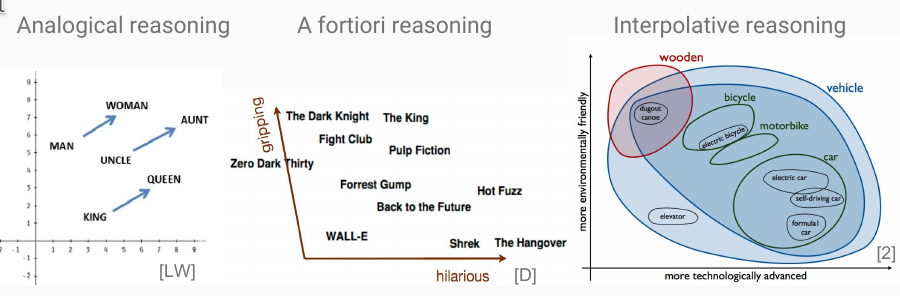
\includegraphics[width=\textwidth]{graphics/stolenfigures/reasoning_samples.png}
	\slcaption{
		Different forms of reasoning represented graphically. \todoparagraph{Holy shit remove me}
	}
    \label{fig:graphic_reasoning}
\end{figure}

To automate these forms of inference, we need a richer form of knowledge than what is available in calssical logic: We need a notion of / Information about \textbf{Betweenness} and \textbf{Directionality}.

To model the stuff in \autocite{fig:graphic_reasoning}, we need a good metric, and what we see there definitely sounds euclidian!

\textbf{Summarized, CS are better than symbolism because we save the inference engine (plus we can extend and simulate knowledge bases with commonsense reasoning, just like humans deal with incomplete knowledge!) and better than connectionism because they are explainable. Klar soweit?!}

\todoparagraph{The problems of polysemy und synonymy for classical stuff, see fundamental information retrieval problem}


% \includeMD{pandoc_generated_latex/2_4_typesofreasoning}

\section{Other Related Work}
\label{sec:otherwork}

This thesis focuses on the aforementioned algorithm, primarily considering \cite{Derrac2015} and on top of that only two follow-up works: \cite{Ager2018, Alshaikh2020}, which have shown to provide useful extensions for it without changing its core logic. This shall by no means mean that these are the only ones that could be considered.

\paragraph{Tag Genome} 

By far the closest to what we do is the algorithm of \textcite{VISR12}, who generate a so-called tag genome for the domain of movies supervisedly based on keywords that users have assigned manually. Their algorithm takes these binary assignments and creates a dense representation that encodes a degree of relevance for each combination of movie and tag. Furthermore, they create a dedicated movie recommendation system on basis of this (interface reprinted in \autoref{fig:movietuner}). This system provides explainable recommendation based on these tags, allowing users to request recommendations for movies such as \textit{\q{I‘d like something less violent than Reservoir Dogs}} \cite[3]{VISR12}. Not only is their application exactly what is being demanded here, but the algorithm itself also performed significantly better than the one of \textcite{Derrac2015} in a human study of the latter, in which they directly compared the techniques by asking subjects which of the respectively extracted keywords better describes the difference between two movies \cite[44]{Derrac2015}. Considering however that \gencite{VISR12} algorithm is supervised and requires data which does not exist for our domain, it cannot be applied in our case. On the contrary, the final results of their algorithm are preferred by users over the ones generated with the algorithm considered in this work, but structurally exactly equal. This provides clear evidence that the desired application of this work is possible, albeit of lower quality than what their work achieved.

Generally, what is being done here corresponds to \textbf{Representation Learning}, whose aim is to discover the inherent semantic structure of a representation unsupervisedly \cite{Dayan1995}. More specifically \textbf{Disentangled Representation Learning}, where only salient attributes relevant to the task at hand should be extracted, which means finding latent embeddings whose dimensions are meaningful interpretable features. Generative Adversarial Networks \cite{Goodfellow2014} or Variational Autoencoders \cite{Kingma2013} are modern techniques that are good at finding latent information in images. Especially InfoGAN \cite{Chen2016} should be named, which can extract interpretable features such as pose, hairstyle, prensence of glasses and emotions from images unsupervisedly. 

\paragraph{LDA} 
\label{sec:lda}

In the realm of \gls{nlp}, this also relates to \textbf{Topic Modeling}, which aims to extract multiple hidden themes from a given text corpus by discovering groups of co-occuring words unsupervisedly. A well-known algorithm for this is Latent Dirichlet Allocation (LDA) \cite{Blei2003}, which represents documents by its salient \textit{topics}, each of which being a cluster of natural language terms. This technique bases on the assumption that each text consists of various topics, which are in turn made up by various keywords, making it possible to represent texts as multinomial distribution over latent topics which are aggregations of these keywords. Assuming a hierachical bayesian distribution where each text of a corpus is represented as mixture of topics it contains, their unsupervised algorithm extracts these by approximating the underlying infinite mixture of topic with an expectation-maximization (EM) algorithm. This yields a representation where each text is explicitly represented by the most propable words according to this distribution for a finite number of most probable topics. The algorithm finds use in text classification and collaborative filtering, but relies on unflexible \gls{bow} representations, making it hard to incorporate additional information such as correlations between topics \cite{Ager2018}.


\paragraph{Academic Interests Recommender}
\label{sec:sidbert}
Regarding the used domain, there is already a system incorporated into the Siddata-\gls{dsa} that aids students by finding and recommending educational resources. SidBERT \cite{Schrumpf2021DELPHI} extracts implicit information from courses and other learning material by their title by categorizing them into one of 905 classes derived from the third or fourth level of the \gls{ddc} \cite{Dewey1876}, a hierachical tree stucture system commonly used to categorize library books. SidBERT uses the same dataset as this work and classifies with a custom classification head ontop of a \gls{bert}-encoder \gls{ann} which is trained on 1.3 million book titles collected from three universities as well as the German National Library, currently achieving 45.2\% test accuracy (62.2\% recall) among 905 classes.

\paragraph{Variations of this Algorithm}
\label{sec:algo_variants}

There are also techniques that extend the algorithm of \textcite{Derrac2015}: \textit{Alshaikh et al.} \cite{Alshaikh2019, Alshaikh2021} use this algorithm as one of their steps and create a similar algorithm to find disentangled features that is in line with the requirement of Conceptual Spaces to consist of low-dimensional domain-specific subspaces. Regarding other unsupervised ways to create Conceptual Spaces, Gärdenfors himself suggested in his book \cite{Gardenfors2000a} to use self-organizing maps (Kohonen-Networks \cite{Kohonen1997}) instead of classical \gls{nlp} algorithms and \gls{mds} to unsupervisedly create concpetual spaces. Finally, the whole concepts of vector-space models for words \cite{Mikolov2013} and texts \cite{Le2014,Devlin2019} is related in that represents the meaing of terms, phrases or documents by embedding them in a vector space. However these have arbitrary non-interpretable dimensions and are no metric spaces, thus having no relation of geometry and meaning for \eg betweeness or analogical reasoning, which will be eloborated in the next section. For more related work it is also referred to the respective sections of \mainalgos.


\section{Relevant Algorithms and Techniques}
\label{sec:required_algos}

\todoparagraph{TODO: term? phrase? n-gram? - check where I mean what}

% \todoparagraph{dont forget the links for lsa und lda - are in lsa-long-md }

Thus far, we have described the base algorithm which this thesis replicates. Before describing each of its step in detail, it is useful to get a grasp of the theoretical foundation that form the basis of the creation of linguistical \glspl{vsm} in general. This also helps to place the algorithm in the context of the field of computational \gls{nlp}. Note that this section primarily serves to understand the key concepts required for the methodology of \textcite{Derrac2015}. To do that, we will sometimes put emphasis on other algorithms of the same type than those actually used in the implementation if they express the model more explicitly. The the methodology is modular and \eg only requires \textit{some} algorithm for dimensionality reduction.

%  also quickly look at what other techniques can be used for some of its components.

\subsection{Classical Vector Space Construction}
\label{sec:vsm_construction}

The methodology in question consists of several components, each of it being an algorithm in itself. The first steps are basically classical linguistic tools: A text corpus is preprocessed and the words of its entites are counted and raw counts transformed. From these values a frequency matrix is generated and its dimensionality is reduced, before directions for domain-specific similarity measures are extracted.

\textcite{Lowe} conceived a general framework to construct vector spaces from texts, splitting the process into the steps of first counting the token frequencies, then transforming the raw counts into more useful \gls{quant} measures %adjust the weights of the elements in the matrix, because common words will have high frequencies yet are less informative than rare words.
 %TODO: talk about a fucking DOC-TERM-MATRIX, A MATRIX OF FREQUENCIES!!!
and smoothing the space using dimensionality reduction, before calculating the similarities on the resulting embedding. While the considered algorithm requires more steps before calculating the similarities to allow for domain-specific and other more complex forms of reasoning, it also adheres to this structure.%, as will be shown in section~\nameparanref{sec:generate_vectorspaces}.

\paragraph{Distributional Semantics}
\label{sec:bow_hypothesis}

\begin{quote}
    \textit{\q{you shall know a word by the company it keeps}} \textcite{firth57synopsis}
\end{quote}

The core principle behind any kind of embedding of linguistics units such as words or documents is the distributional hypothesis, which states that linguistic items with similar distributions have similar meanings. If this is the case, the meaning of words correlate with their distribution: Words that occur in similar surroundings have similar meanings.

More precisely, vector-space models fall into different categories depending on if the similarity of documents (\textit{Term-Document-Model}) or of words (\textit{Word-Context-Model}) is in question. Because the algorithm considered here describes the relation of entites through their descriptions it falls unser the latter category. According to \textcite{Turney2010}, the assumption underneath the Term-Document model is more precisely called the \textbf{bag-of-word hypothesis}, which states that documents with similar distributions of words have similar meaning. Accordingly, when embedding documents into a vector space, it must be ensured that the similarity relations of the embeddings closely resemble the similarity of the original documents.

Many \gls{nlp} tasks rely on documents being represented as vectors, such as Information Retrieval, Recommendation, Text Classification, Translation, Sentiment Analysis and many more \cite{Smith2017,bird2009natural,Devlin2019,Le2014,Mikolov2013a,Turney2010,Guo,Chen2018,Maas2011}. The process of turning a collection of texts document into numerical feature vectors is referred to as \textit{vectorization}. According to \textcite{Turney2010} (who base their work on \textcite{Lowe}), the construction of a \gls{vsm} from texts can be decomposed into a four steps:\footnote{When considering neural embeddings such as \gls{word2vec}, the separation of these steps is hidden in the algorithm and not as distinct, but the principles hold also in these techniques.}

% \todoparagraph{zu 90 prozent raus hiermit, und falls doch drin dann kleiner}
% \begin{quote}
% 	\q{After the text has been tokenized and (optionally) normalized and annotated, the first step is to generate a matrix of frequencies. Second, we may want to adjust the weights of the elements in the matrix, because common words will have high frequencies, yet they are less informative than rare words. Third, we may want to smooth the matrix, to reduce the amount of random noise and to fill in some of the zero elements in a sparse matrix. Fourth, there are many different ways to measure the similarity of two vectors.} \hfill \textcite{Turney2010}
% \end{quote}

\begin{description}
    \item[1) Building the Frequency Matrix] which starts with preprocessing such as tokenization followed by normalizing and possibly \gls{lemma}tizing the tokens amongst many other possible techniques, before counting frequencies of either words or \glspl{ngram}, yielding a matrix of \glspl{bow}.
    \item[2) Transforming Raw Frequency Counts] \q{[B]ecause common words will have high frequencies, yet they are less informative than rare words} \cite{Turney2010}, it may make sense to adjust the weights of the elements of the frequency matrix such that the distances are not distorted by them.
    \item[3) Smoothing the Frequency Matrix] A matrix that counts the frequency of any word in the corpus is generally noisy, sparse and extremely high-dimensional. Dimensionality Reduction helps to counter all three issues, yielding vectors closer resembling the document's \textit{latent information}.
    \item[4) Calculating Similarities] of individual vectors is the final step and aim of most embedding algorithms. This can be done in various ways, a classical technique is to use their \gls{cos}.
\end{description}

Importantly, our algorithm differs from this four-step-process by injecting several additional steps before calculating similarities. This is because we hold the notion that similarity is necessarily context-dependent and there is no overall similarity (see \autoref{sec:reasoning}), which requires additional dissection of this step. In the following, we will describe three steps relevant for us.


\subsubsection{1. Bag-of-ngrams representation}
\label{sec:techniques:bow}

The most relevant information that can be taken into account when comparing two texts are the words they consist of. Accordingly, an obvious choice to vectorize a collection of documents is to describe each document the counts of its word occurences, which is called \gls{bow}-representation. 

This approach is simple but has important drawbacks: Firstly, a document is not fully described only by the words it contains but also specifies their constellation. The information about ordering and relative position is lost in this representation (consider not knowing the position of negations). To alleviate this issue, texts can instead be represented as glspl{n-grams}, where the tokens are not single words but all sequences of words of length $n$. The drawback is that this vastly increases sparseness and dimensionality.

Further, by representing each word as separate \textit{one-hot-vector} ignores word semantics: as every vector is equally distant from any other, synonyms (cases where the same meaning is expressed with different words) are just as far apart as antonyms (opposites). This unreliability of term-document-association is what \textcite{Deerwester} calls the \textit{fundamental information retrival problem}: The mapping between words and their meanings is not bijective, but ambiguous. Different words can be used to express the same concept, and sometimes the same word refers to different concepts. This issue is partially alleviated by the dimensionality reduction performed subsequently, which may provide a way to determine what concepts are implied and obfuscated by fallible word choice.

To address both issues, modern algorithms exist that train a document embedding directly based on constellation (alleviating lost ordering) of word-embeddings that are pre-trained based on their usual context (alleviating distance relation problems)
. \todoparagraph{But later.}

\subsubsection{2. Word-weighting techniques}
\label{sec:word_count_techniques}

When comparing the \gls{bow}-representations of texts, it is reasonable to give more weight to \emph{surprising} words than to expected ones. The idea behind that is, that \q{surprising events, if shared by two vectors, are more discriminative of the similarity between the vectors than less surprising events.} \cite[156]{Turney2010} Another crucial reason is, that individual texts in the corpus are of drastically varying length, so longer entities would naturally dominate shorter ones when only comparing the raw counts - considering relative frequencies instead of absolute ones alleviates such problems. The algorithms explained below transform the raw frequency-counts of a document and an \gls{ngram} into some \emph{score}, dependent on the number of occurences of this term in this document as well as the counts of other \glspl{ngram} and other documents. This score is henceforth called a \gls{quant}.

Let us consider term $t$, corpus $C$, document $d \in C$ (represented as \gls{bow}). Then:\\
term-frequency $\text{tf}_{t,d}$: How often $t$ occurs in $d$\\
document-frequency $\text{df}_t$: How many documents $\in C$ contain $t$\\
summed term-frequency $\text{df}_{t,*} = \sum_{d' \in C} \text{tf}_{t,d'}$: How often $t$ occurs in any document $\in C$

\paragraph{Tf-Idf} The most well-known technique formalizing this concept is \gls{tf-idf}, which gives a term-document pair a higher weight if the term is generally rare in the corpus (low \textit{df}) and frequent in the respective document (high \textit{tf}):
\vspace{-2.3ex}
$$ w_{t,d} = \text{\textit{tf}}_{t,d} * log(\frac{|C|}{df_t}) $$

%see also: https://towardsdatascience.com/3-basic-approaches-in-bag-of-words-which-are-better-than-word-embeddings-c2cbc7398016
%\cite{Turney2010} (sec 4.2): Salton and Buckley (1988) defined a large family of tf-idf weighting functions and evaluated them on information re- trieval tasks, demonstrating that tf-idf weighting can yield significant improvements over raw frequency

\paragraph{PPMI}
% See also: https://stackoverflow.com/a/58725695/5122790

\textcite{Turney2010} suggested to use the \gls{ppmi} measure instead of \gls{tf-idf} to weight the counts in \glspl{doctermmat}, relying on \cite{Bullinaria2007}'s work taking into account psychological models to extract information about lexical semantics from co-occurence statistics. According to these works, \gls{ppmi} performs most plausible to measure semantic similarity in word-context matrices compared to human evaluation. For that reason, \textcite{Derrac2015} and its follow-up works \cite{Ager2018,Alshaikh2020} rely solely on this technique. %(sec 4.2) of \cite{Turney2010}: Bullinaria and Levy (2007) demonstrated that PPMI performs better than a wide variety of other weighting approaches when measuring semantic similarity with word-context matrices.
Like tf-idf, it weights terms that are strongly associated with a document highly by favoring terms frequently associated with document $d$ while infrequent in the corpus overall. For that, it uses the logarithm of the probability of the considered term-document-combination $d,t$, normalized by the probability of this document co-occuring with any term ($d,*$) and this term co-occuring with any document ($t,*$)
\vspace{-2.2ex}
\begin{align*}
   w_{t,d} &= max\left(0, log\left( \frac{p_{d,t}}{\sum_{t'}p_{d,t'}*\sum_{d'}p_{d',t}} \right) \right) \\
   p_{d,t} &= \frac{\text{tf}_{t,d}}{\sum_{d'}\sum_{t'} \text{tf}_{t',d'}}
\end{align*}


\subsubsection{3. Dimensionality Reduction and Latent Space Embedding}
\label{sec:dim_red}

At this step, we have a sparse and high-diensional matrix quantifying the importants of all corpus-terms for all documents. The next step is to smooth this frequency matrix. Reducing the dimensionality of this matrix reduces computational processing load and helps in alleviating the prevalence of irrelevant noise in the original matrix \cite{Turney2010}. Additionally, the right algorithms may also make use of the principles of distributional semantics to alleviate the aforementioned problems of word distance and synonymy. The result is that the document vectors depend less on their exact phrasing and instead more closely resemble the concepts that these words expressed, also called its \textit{latent} (hidden) \textit{topics}. This may even improve subsequent similarity measurements, as it is less distorted by noise and word choice irregularities.

%TODO: we said in bow-representation that LSA helps with the fact that the same thing can be expressed in different ways
% We start with sparse vectors, and then \q{some form of dimensionality reduction is typically used to obtain vectors whose components correspond to concepts.} \cite{Derrac2015}

The technique that most explicitly models a document's latent topics is \gls{lsi} \cite{Deerwester}, which relies on the fact that words that are close in meaning will occur in similar pieces of text to yield embeddings where words and documents of similar meaning are similar. 

\paragraph*{LSI/LSA\footnote{Both terms refer to the same algorithm, which is generally called \gls{lsi} when applied to document similarity and information retrieval, and \gls{lsa} when applied to word similarity.}}

While language is used to express the world, it is also highly ambiguous and redundant, such that the relationship of model and reality is only a statistical one. The same thing can be expressed with different words (synonymy), and sometimes a word has different meaning depending on context (polysemy). The underyling latent semantic structure in texts is obscured by the randomness of word choce, such that individual words provide only unreliable evidence about the conceptual topic or meaning of a document.
% When comparing two texts (text and query, ...) what we have are the words which are only a sample descrption of the underlying conceptual/semantic context.

However, language has a lot of structure, which allows to treat this as statistical problem: The occurrence of some patterns of words gives a strong clue as to the likely occurrence of others. According to the distributional hypothesis, the matrix of observed occurrences of terms applied to documents can be used to estimate parameters of the underlying true model. This is explicitly done using linear algebra operations on the frequency matrix in \gls{lsi} \cite{Deerwester}. 

This algorithm decomposes the \gls{doctermmat} into a product of three linearly independent factors: \textit{words-per-topic} \texttimes \textit{topic-importance} \texttimes \textit{corpus-topic-distribution}. Then it runs \textit{Truncated Singular Value Decomposition} (SVD), which finds a lower-rank approximation of the matrix containing the \textit{hidden information} while identifying and keeping relationship patterns. In other words, by taking only the important components from this matrix (\textit{rank-reduction}), the new representation becomes lower-dimensional, less noisy and less sparse, but still approximates the original similarity behaviours.

LSI explicitly represents both documents and terms in the same semantic space, such that they are treated equally when the SVD analyses their similarity behaviour. It yields a representation of arbitrary dimensionality that captures the relation of term-term, term-document and document-document similarity by ensuring that similar items will end up close in the space. Importantly, this yields a representation in wich both documents and terms correspond to vectors. The similarity of each of these is assessed via the cosine-distance. To analyze the similarity of a document and a query term, the term is embedded by generating \textit{pseudo-document} (a document that contains only this term), and close vectors are returned, which may include results that conceptually similar but do not share any words. 

As consequence of the compression, some dimensions are combined and depend on more than one term - generally this merges embeddings of similar terms, mitigating synonymy. Also Polysemy is reduced, as only the components of polysemous words that have encode a similar meaning than the cluster are relevant for the combined direction of the vector. Another consequence is that terms that did not actually appear in a document may still end up close to the document, if that is consistent with the major patterns of association in the data: Terms that \textit{could} have been used as well.\q{if the tags \textit{love story} and \textit{hilarious} have been applied to an item, it is likely that the tag \textit{romantic comedy} is highly relevant\cite{VISR12}.}

The algorith to create the Tag Genome in \cite{VISR12} bases to a high degree on this algorithm: It creates a binary frequency matrix for all considered documents and a set of \textit{tags}, embeds documents and pseudo-documents generated from the tags and compresses it with LSI. The relevance of a tag for a documents \codefunc{tag-lsi-sim(t,i)} is then calculated by their embeddings' cosine similiarity. Also, the algorithm appears to be a good method to find clusters of similar terms for semantic direction, given that it considers these terms as directional vectors already. 

\textcite{Derrac2015}, however, additionally require that spatial relations such as betweeness and parallelism hold in the vector space embedding. For that, they require a space of Euclidean metric which is not given in LSA, which generates a space based on the similarity-centred objective to reduce \glspl{cos} of similar entites. Instead they follow \textcite{Gardenfors2000} suggestion and rely on \gls{mds}. While the algorithm bases on Euclidean distance, the principle that items of similar meaning will end up in similar positions still holds. In fact, it should hold most kind of compression, bearing in mind the distributional hypothesis and the fact that if there is some inherent \textit{structure} (obfuscated by wording) that explains the dissimilarity of any text corpus sufficiently well, it will remain after the compression.

\paragraph*{Multi-dimensional Scaling}
\label{sec:mds}

\Gls{mds} \cite{Mead1992} is a dimensionality reduction technique that induces a finite vector-space representation from pairwise similarities. It takes a \gls{dissimmat} as input and returns a fixed-dimensional embedding in which original distances are kept as close to the ones of the \gls{dissimmat} as possible. Gärdenfors considered using this technique it to find an underlying \textit{phenonemal} conceptual space from human similarity judgements, given that it yield q{as high a correlation as possible between the similarity judgements of the subjects and the corresponding distances in the estimated dimensional space} \cite[22]{Gardenfors2000a}. The algorithm has quadratic space complexity \cite{Alshaikh2021}

Especially relevant is the \textit{metric MDS} algorithm, which requires metric distances as input and models their similarity as distances in a space finite space of lower dimensionality with a Euclidean metric. A distance measure is a metric if the following axioms hold:
\vspace{-2ex}
\begin{align}
    d(x,y) = 0 &\Leftrightarrow x = y \\
    d(x,y) &= d(y,x) \\
    d(x,t) &\leq d(x,y) + d(y,z) \text{ (triangle inequality)}
\end{align}

Given metric distances $d(p_i, p_j) \forall 1 \leq i, i \leq j$ and the demanded number of dimensions k, the algorithm starts with a random initial distribution and progressively adjusts the coordinates by re-computing the embeddings $v_1, ..., v_n \in \mathds{R}^k$ such that distances are maintained as well as possible by minimizing 
\vspace{-2ex}
$$ \sum_{i=1}^{n-1}\sum_{j=i+1}^{n}(d(p_i, p_j) - \lVert v_i - v_j \rVert)^2 $$

\removeMe{
\subsection{Other important Techniques}


\includeMD{pandoc_generated_latex/2_othertechniques}

\subsubsection*{Semantic Knowledge Bases}

Lexical databases of semantic relations between words, the most famous of which being WordNet,\footnote{\url{https://wordnet.princeton.edu/}} link words in a graph that encodes explicit semantic relations like synonyms and hyponyms (subtypes/ \emph{is-a}-relationships). While neural %TODO: nicht neural, aber halt data-driven? naja das was word2vec undso sind... by-context-created/trained...?! similarity-based? -> DISTRIBUTIONAL MODELS (ones trained from the co-occurrence patterns of temrs)
embeddings may encode similar information implicitly, when relying on dictionary-based word encodings they are an important tool when using classical linguistic techniques. For the developed algorithm, the information how many hyponyms of a candidate word for a semantic direction %TODO: did I explain the algorithm well enough before this to throw this much information at the reader?!
occur in its corresponding text-corpus can be highly relevant. To do that, WordNet \cite{Miller1995} and it's German equivalent, GermaNet \cite{hamp-feldweg-1997-germanet,Henrich},\footnote{\url{(https://uni-tuebingen.de/fakultaeten/philosophische-fakultaet/fachbereiche/neuphilologie/seminar-fuer-sprachwissenschaft/arbeitsbereiche/allg-sprachwissenschaft-computerlinguistik/ressourcen/lexica/germanet-1/)}} are used in the respective step.

}